\chapter{Background}

The reader of this thesis is likely to know Haskell very well
and read this thesis to understand the GHC stack (chapter~\ref{chp:the_execution_stack}) or to understand the stack traces
proposal of this thesis (chapter~\ref{chp:reifying_the_stack}
and~\ref{chp:a_haskell_interface}). However, this thesis must be
approachable to my fellow class mates according to the thesis
regulations at Chalmers. That includes students with almost no prior
Haskell knowledge. Haskell is a big language with many aspects and it
takes many years to master. Therefore, the Haskell background which is
in section~\ref{sec:haskell} focuses on what is going to be essential to
understand \emph{this} thesis.

\section{Stack traces}

When a computer program crashes, the runtime of some programming languages
gives some context to where in the code the program crashed.
Typically, a \emph{stack trace} is printed. A stack trace is the listing
of the functions that have called each other and have not exited yet, so
they have all been part of the crash. The first function in the stack
trace is always the program entry point, the last function is where the
crash actually occurred.

The Rosetta Code wiki contains a code sample in Ruby illustrating a stack
trace \cite{rosetta_stone_st}, reproduced here in figure~\ref{fig:ruby_stack_trace}. As the figure shows, some languages can print stack
traces at any time, not only after crashes. Stack traces can not be
implemented as a regular user-level library, stack traces will need
to look at the internal state of the run time system or interpreter.
In the case of Ruby, they have the magical primitive \texttt{caller} which
retrieves the call chain. It would not be possible for a user
to implement \texttt{caller} in pure Ruby. To implement stack traces
in Haskell is no exception, the implementation we present in this work
will need to look at the internal state of the runtime system and has to
target a specific Haskell compiler. The compiler we target is GHC.

\begin{figure}
\begin{mdframed}
  \begin{subfigure}[t]{0.5\textwidth}
      \begin{minted}{ruby}
def outer(a,b,c)
  middle a+b, b+c
end

def middle(d,e)
  inner d+e
end

def inner(f)
  puts caller(0)
  puts "my arg is #{f}"
end

outer 2,3,5
       \end{minted}
    \caption{Ruby code printing a stack trace.}
    ~ %add desired spacing between images, e. g. ~, \quad, \qquad etc.
    %(or a blank line to force the subfigure onto a new line)
  \end{subfigure}
        \begin{subfigure}[t]{0.5\textwidth}
          \begin{verbatim}
$ ruby stacktrace.rb
stacktrace.rb:10:in `inner'
stacktrace.rb:6:in `middle'
stacktrace.rb:2:in `outer'
stacktrace.rb:14
my arg is 13
          \end{verbatim}
          \caption{Output of running the Ruby program.}
        \end{subfigure}
        \caption{Illustration of a simple stack trace.}
        \label{fig:ruby_stack_trace}
\end{mdframed}
\end{figure}

\section{Haskell} \label{sec:haskell}

Haskell is a lazy, functional, general-purpose programming language \cite{haskell_report2010}.
Haskell first appeared in 1990 \cite{HistoryOfHaskell2007} and has since
released the major standards Haskell 98 and Haskell 2010
\cite{haskell_report2010}.

\begin{figure}
\begin{mdframed}
  \begin{minted}{haskell}
main = print (fibonacci 10)

fibonacci :: Int -> Int
fibonacci 1 = 0
fibonacci 2 = 1
fibonacci x = fibonacci (x - 1) + fibonacci (x - 2)
  \end{minted}
  \caption{A simple Haskell program.}
  \label{fig:simple_program}
\end{mdframed}
\end{figure}

Figure~\ref{fig:simple_program} shows a simple program in Haskell.
Two functions are defined in this program, \texttt{main} and
\texttt{fibonacci}.  The explicit type signature for the function
\texttt{fibonacci} means that it takes an int and returns an int. If a type
signature is omitted, like for \texttt{main}, Haskell will infer it automatically.

\subsection{Error handling in Haskell} \label{sec:error_handling_in_haskell}

In order for stack traces to be relevant for a programming language, programs
must have the notion of \emph{crashing}. Intuitively, crashing causes sudden
stops in execution, either by the operating system or by the language's own
exception handling. Program crashes can be disastrous, since they will also
terminate processes that are supposed to be long-running. Hence there are
language constructs to eliminate some causes of program crashes.
For instance,
evaluating a well-typed expression in Haskell can not segfault \cite{FindingTheNeedle2009}.

In theoretical computer science, there's a notion of a function being \emph{total}. Meaning
that a function will terminate and not return any error. Therefore,
such a function can not crash. Unfortunately, as of the famous halting
problem it's not possible to decide if a function will terminate or not.
That implies that you can't in general
verify that a function is total \cite[p.380]{Hopcroft:2000}.
The good news, though, is that whenever we
explicitly \emph{choose} to crash, we can systematically avoid it. This is not
only true in the language Haskell, Java implements this through the
\texttt{throws} keyword \cite{oracle_java_doc_method_throws}. 
To annotate the function signature with \texttt{throws ArithmeticException}
would mean that the function may throw an \texttt{ArithmeticException}.
Figure~\ref{fig:total_java} shows a Java integer division function that
is total.

\begin{figure}
\begin{mdframed}
  \begin{subfigure}[t]{1\textwidth}
      \begin{minted}{java}
int integerDivision (int nom, int den) throws ArithmeticException {
  if (den == 0) {
    throw ArithmeticException("Division by zero");
  }
  else {
    return nom / den;
  }
}
       \end{minted}
    \caption{A total function in Java.}
    \label{fig:total_java}
  \end{subfigure}
        \vskip2em
        \begin{subfigure}[t]{1\textwidth}
          \begin{minted}{haskell}
integerDivision :: Int -> Int -> Maybe Int
integerDivision n 0 = Nothing
integerdivision n d = Just (n `div` d)
          \end{minted}
          \caption{A total function in Haskell.}
          \label{fig:total_haskell}
        \end{subfigure}
        \caption{Two total functions.}
        \label{fig:total_functions}
\end{mdframed}
\end{figure}


In Haskell, the most common way to implement ``safe'' division is to return the
special value \texttt{Nothing} instead of dividing by zero. To do this in
Haskell, the \emph{Maybe} wrapper must be put in the function signature. See
figure~\ref{fig:total_haskell}.

The two functions in figure~\ref{fig:total_functions} will not crash when dividing
by zero, rather, they gracefully return a value of either the division or a
value representing failure. But there's a drawback, both these functions are
cumbersome to use. In Java the programmer needs to explicitly catch the
Exception combining the \texttt{try} and \texttt{catch} constructs
\cite{oracle_java_doc_compile_time_checking_of_exceptions, oracle_java_doc_catch}.
In Haskell, an additional layer of pattern
matching is required. Due to this inconvenience, both languages allow
for carrying out integer division without forcing the caller to do any
error handling. Figure~\ref{fig:partial_functions} shows two partial
functions. Partial functions are controversial in Java
\cite{oracle_java_doc_controversy} and discouraged when unnecessary in
Haskell \cite{haskellwiki_avoiding_partial_functions}.

\begin{figure}
\begin{mdframed}
  \begin{subfigure}[t]{1\textwidth}
      \begin{minted}{java}
int integerDivisionUnsafe (int nom, int den) {
  return nom / den;
}
      \end{minted}
    \caption{A partial function in Java.}
    \label{fig:partial_java}
  \end{subfigure}
        \vskip2em
        \begin{subfigure}[t]{1\textwidth}
          \begin{minted}{haskell}
integerDivisionUnsafe :: Int -> Int -> Int
integerDivisionUnsafe n 0 = error "Division by zero"
integerDivisionUnsafe n d = n `div` d
          \end{minted}
          \caption{A partial function in Haskell.}
          \label{fig:partial_haskell}
        \end{subfigure}
        \caption{Two partial functions.}
        \label{fig:partial_functions}
\end{mdframed}
\end{figure}

For the first time we now see the \texttt{error} function in Haskell (figure~\ref{fig:partial_haskell}).  \texttt{error} is a
special built-in function that terminates execution and outputs the provided
message. While it's not entirely accurate, we could think of \texttt{error}
being the only gateway to crashing a Haskell program. That means that all the
typical dangerous operations like integer division by zero or indexing outside
an array would just invoke the \texttt{error} function. We define ``crashing''
to be whenever \texttt{error} is called.

The conclusion is that Haskell has two major types of error
values \cite{o2008real} \cite{ezyang_8_ways_to_report_errors}, errors in total functions (figure~\ref{fig:total_haskell}) and errors in partial functions (figure~\ref{fig:partial_haskell}). In this thesis we only care about the
latter.

\subsection{Functional Programming Concepts}

The language that we want to add stack traces to is a lazy functional
programming language. It is important to be aware of this when
implementing stack traces for Haskell. In this subsection we will look
at how Haskell expressions are evaluated. The concepts presented here
is fundamental knowledge in Haskell programming.

\subsubsection{Equational Reasoning}

We will not go into details of how the Haskell language specification
defines evaluating an expression, but there is no concept of a
entering a function then let it return. Instead you think of it
as successively applying equations until you reach a completely
evaluated value. Applying an equation having the form $lhs = rhs$ on an
expression means to substitute $lhs$ in the expression to $rhs$, figure~\ref{fig:equational_reasioning} shows this by example.
To understand equational reasoning is helpful when learning Haskell.

\begin{figure}
\begin{mdframed}
  \begin{minted}{haskell}
-- We can define a few functions (or equations)
f x = g x + h x
g x = 5 + h x
h x = x + 2

-- If Haskell is evaluating a value like (f 10), you can apply the
-- equations from above and reach the same result as your Haskell
-- program would.
f 10                  ==> -- equation for f
g 10 + h 10           ==> -- equation for g
(5 + h 10) + h 10     ==> -- equation for h
(5 + (10 + 2)) + h 10 ==> -- (+) (we treat it as a primitive)
(5 + 12) + h 10       ==> -- (+)
17 + h 10             ==> -- equation for h
17 + (10 + 2)         ==> -- (+)
17 + 12               ==> -- (+)
29                        -- Done!
  \end{minted}
  \caption{Haskell can be understood by equational reasoning.}
  \label{fig:equational_reasioning}
\end{mdframed}
\end{figure}

\subsubsection{Recursion and Tail Calling}

Haskell has no statements, only expressions\footnote{Haskell has no statements,
  but the code can be in an imperative looking style when using the
  \texttt{do}-syntax}. So obviously there
can be no loop-statements like the \texttt{for}-statement or
\texttt{while}-statement. As a general purpose language,
Haskell naturally has a replacement for loops, namely \emph{recursion}. Figure~\ref{fig:tail_call_fun} shows two implementations of the mathematical
function $ fun(limit, acc) = acc + \sum_{x=1}^{limit}{x} $, one in
Haskell and one in the imperative language C.

\begin{figure}
\begin{mdframed}
        \begin{subfigure}[t]{0.5\textwidth}
            \begin{minted}{haskell}
fun acc 0     = acc
fun acc limit =
  fun (acc + limit)
      (limit - 1)
            \end{minted}
            \caption{Haskell version. Implemented with recursion.}
        \end{subfigure}
        ~ %add desired spacing between images, e. g. ~, \quad, \qquad etc.
          %(or a blank line to force the subfigure onto a new line)
        \begin{subfigure}[t]{0.5\textwidth}
          \begin{minted}{c}
// 'acc' is like a start-value
int fun(int acc, int limit) {
  while (limit != 0) {
    acc   = acc + limit;
    limit = limit - 1;
  }
  return acc;
}
          \end{minted}
          \caption{C version. Implemented with loops.}
        \end{subfigure}
        \caption{Two functions.}\label{fig:tail_call_fun}
\end{mdframed}
\end{figure}

When recursion is used as a replacement for loops in C programming, it
is often a poor choice. Recursion uses stack space,
it needs to save both local variables and a return address on the stack
for each function call. But this is not always true, in some cases it
is possible for the compiler to optimize the recursive code into code
using loops! This optimization is called \emph{tail call optimization}.
For functional programming languages, this optimization is of utmost
importance, as recursion is the standard way of doing control flow.
A tail call is a like a regular call, only that the caller is
replacing its current stack frame instead of creating a new stack frame.
The insight is that if a call will not return to the calling function (say
if the call is the last statement), it is safe to overwrite the current
stack frame.

In Haskell, the intuition is the same, but the technical explanations
don't carry over. There are no statements, so there is no notion of a
last statement. In chapter~\ref{chp:the_execution_stack} we will see how
function calls and jumps in Haskell are implemented for the Glasgow
Haskell Compiler.

\subsubsection{Purity}

Haskell is a \emph{pure} language where functions do not have side
effects and this is a good consequence of equational reasoning. So any
function \texttt{fun} can be run twice with the same arguments and will
always return the same value. There will also be no side effects of
running it twice. From figure~\ref{fig:purity_er} we see that purity is
a necessity for equational reasoning. Note how the first step is turning
\emph{one} occurrence of \texttt{g} into \emph{two} occurrences by
applying the equation for \texttt{f}. If running \texttt{g} would have
had side effects, this would not have been possible.

\begin{figure}
\begin{mdframed}
  \begin{minted}{haskell}
-- Equations:
f x = x + x
g y = y + 3

-- Let's evaluate (f (g 10))
f (g 10)          ==> -- equation for f
(g 10) + (g 10)   ==> -- equation for g
(10 + 3) + (g 10) ==> -- (+)
13 + (g 10)       ==> -- equation for g
13 + (10 + 3)     ==> -- (+)
13 + 13           ==> -- (+)
26                ==> -- Done!
  \end{minted}
  \caption{A pure language is a requirement for equational reasoning.}
  \label{fig:purity_er}
\end{mdframed}
\end{figure}

\subsubsection{Laziness}

The critical reader would question why equational reasnoning evaluates
expressions from the outside like we do in figure~\ref{fig:purity_er}.
When expanding the equation for \texttt{f} we get two occurrences of
\texttt{(g 10)}. Why did we not evaluate \texttt{(g 10)} first? It
would have reduced the number of evaluation steps since we evaluate
\texttt{(g 10)} to \texttt{13} and then continue by evaluating
\texttt{(f 13)}. It would have worked in this case, but we can not
in general reduce \texttt{(f (g 10))} to \texttt{(f 13)}. That would
violate the \emph{laziness} property of the language. Another phrasing
for using this evaluation strategy is that Haskell does \emph{outermost
reductions}.

Figure~\ref{fig:laziness} shows an expression that must be evaluated
with lazy evaluation. A strict evaluation strategy would evaluate the
arguments before applying the equation for \texttt{myIf}, leading to a
crash instead of \texttt{5}.

\begin{figure}
\begin{mdframed}
  \begin{minted}{haskell}
-- Equations:
myIf True  onTrue onFalse = onTrue
myIf False onTrue onFalse = onFalse
crash = error "scary side effect!"

-- Let's evaluate (myIf False crash (2 + 3))
myIf False crash (2 + 3) ==> -- equation for myIf
2 + 3                    ==> -- (+)
5                        ==> -- Done!
  \end{minted}
  \caption{Laziness is not an implementation detail, it is a mathematical necessity.}
  \label{fig:laziness}
\end{mdframed}
\end{figure}


\subsubsection{Thunks}

But how do we then ensure that we only evaluate \texttt{(g 10)} once?
Any sensible Haskell implementation will not evaluate \texttt{(g 10)} twice like in figure~\ref{fig:purity_er}.
The solution is to substitute \texttt{(f (g 10))} with \texttt{(f
t) where t = (g 10)} where \texttt{t} is a \emph{thunk}. Figure~\ref{fig:thunks_er} shows the same value being evaluated as in figure~\ref{fig:purity_er} but with thunks. Note that it requires fewer steps
to do evaluation with thunks. Haskell (in most compilers, in most cases)
uses this improved evaluation strategy with thunks, this evaluation
strategy is called \emph{outermost reductions with graph reduction}
\cite{wikibooks_graph_reduction}.

\begin{figure}
\begin{mdframed}
  \begin{minted}{haskell}
-- Let's evaluate (f (g 10))
f t
  where t = (g 10) ==> -- equation for f
t + t
  where t = (g 10) ==> -- equation for g
t + t
  where t = 10 + 3 ==> -- (+)
t + t
  where t = 13     ==> -- (+)
26                 ==> -- Done!
  \end{minted}
  \caption{Equational reasoning with thunks.}
  \label{fig:thunks_er}
\end{mdframed}
\end{figure}

\section{Glasgow Haskell Compiler}

The Glasgow Haskell Compiler (GHC) is a Haskell2010 compatible compiler
\cite{ghc_website}. With it you can compile Haskell source code to an executable
binary. Here's an invocation of the compiler on the program sample from figure~\ref{fig:simple_program}.

\begin{minted}{bash}
  $ ghc --make Fibonacci.hs
  ...
  $ ./a.out
  34
\end{minted}

GHC as of today supports many features in addition to the Haskell2010
standard, like parallelism, many optimizations, a LLVM backend, profiling
and more \cite{ghc_website}.

\subsection{The stack in GHC} \label{sec:stack_in_GHC}

Most programmers have a decent picture of how programming languages
implement functions. Whenever a function is called, its arguments are
pushed on the stack by the caller and the caller jumps to the function's
code. When the function finally exits, it returns to where it was called
from and pops the stack arguments\footnote{Whether if the caller or the callee
should pop the arguments will depend on the \emph{call convention}, but
we do not need to worry about it here.}.  This was a short reminder of how
the \emph{regular stack} works. Most programming languages use this to
implement functions.

Due to the nature of Haskell, it is not clear if the stack that worked
so naturally for languages like C can be used to implement Haskell.
How does it work with partial applications? How does it work for
laziness? Instead one might look at creating a completely new execution
machine. The \emph{Spineless Tagless G-Machine} (STG) from
\cite{stg_1992} is implemented in GHC \cite{evalapplyjfp06} in the sense
that Haskell is compiled down to the STG language at some point during compilation.
The STG machine has a stack called the \emph{execution stack}. The details
of the execution stack changes as new versions of GHC are released.
We have documented the execution stack in chapter~\ref{chp:the_execution_stack} by examining the source code of
the 7.6.2 version of GHC.

\subsection{The runtime system}

Many implementations of programming languages have a run time system
(RTS) and GHC has a run time system too. The RTS in GHC is written
mostly in C. The feature list is long, but the rule of thumb is that
things that can not be implemented in pure Haskell are implemented
in the run time system. Some examples include garbage collection,
an implementation of arrays, synchronization primitives, Software
Transactional Memory, green threads and actual parallelization
\cite{commentary_rts}.

In this thesis, the C-code usually pertains to code from the run time
system. When we say that control is passed from Haskell-land to C-land,
we mean that some Haskell code have called a primitive function that is
implemented in the RTS.

\section{From source to machine code}

Typically, compilers take source code and convert it to machine code.
It would be overwhelming to go directly to machine code, instead most
compilers have some intermediate representations (IR) in the pipeline \cite[p.358]{aho2007compilers}.  For GHC, the pipeline is illustrated in
figure~\ref{fig:ghc_phases} \cite{terei2009low}, the figure only
includes the native code (assembly) backend. Throughout this thesis we will ignore the
C and LLVM backend entirely.

\begin{figure}
\begin{mdframed}
  \centering
  \includegraphics[width=5.5in]{build/fig/phases}
  \caption{The GHC phases of compilation. The LLVM and C backend are not
    shown.}\label{fig:ghc_phases}
\end{mdframed}
\end{figure}

\subsection{The intermediate representations in GHC}

Figure~\ref{fig:ghc_phases} only showed the names of the phases. To
give a rough idea of how each intermediate representation might look
like, we compiled a very small Haskell program with \texttt{ghc} passing
the flags \texttt{-ddump-parsed -ddump-simpl -ddump-stg
-ddump-cmm -ddump-asm}. The output is too verbose to reproduce in
full, instead figure~\ref{fig:recastings} shows some interesting excerpts. Naturally, the
IRs closer to the hardware (Cmm and assembly) will contain more
code and have therefore been truncated much more in figure~\ref{fig:recastings}.

\begin{figure}
\begin{mdframed}
  \centering
  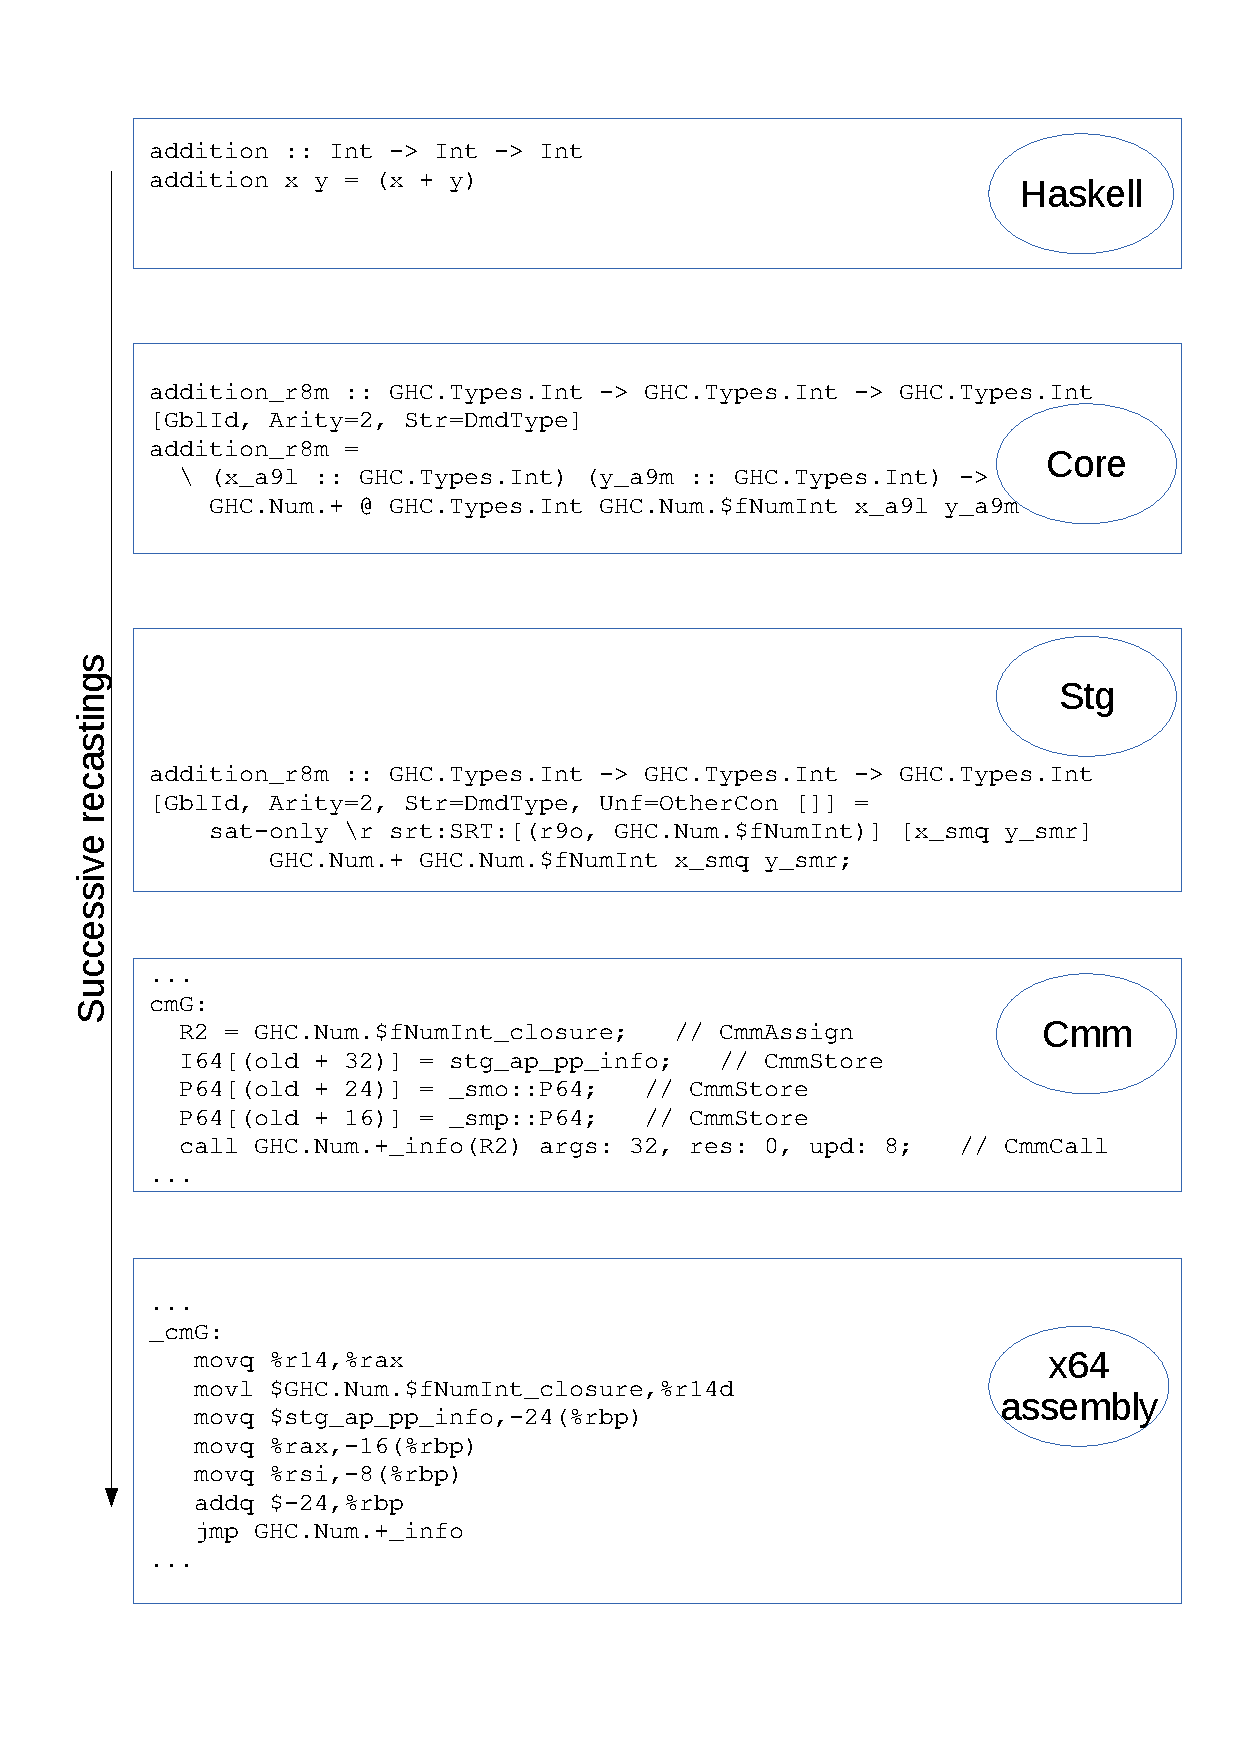
\includegraphics[width=5.5in]{fig/recastings}
  \caption{The IRs in GHC for a simple function. The assembly is also
  included even though it is not an intermediate representation (it is
  the final representation).}\label{fig:recastings}
\end{mdframed}
\end{figure}

\subsubsection{The STG IR}

There is nothing that says that Haskell must be implemented using some
sort of stack. In section~\ref{sec:stack_in_GHC} we saw that GHC, one
popular Haskell compiler, chooses to implement the language using a
stack called the execution stack. The STG intermediate representation
in GHC is interesting to us since it is a representation of code where
it is specified how it will interact with the execution stack \cite{stg_1992, evalapplyjfp06}. The STG
code in~\ref{fig:recastings} does not have a clean syntax, instead we
use the syntax from the Ministg project \cite{haskellwiki_ministg}.
Figure~\ref{fig:haskell_vs_ministg} shows Haskell code and the
corresponding Ministg code. In the Haskell world, \texttt{doubleAddition} and
\texttt{globalThunk} are both just values, in theory we do not really
know if multiple uses of \texttt{globalThunk} will be memoized. Such
implementation details are not relevant in the Haskell world.
Looking at the STG however, we can be sure whether the value
\texttt{globalThunk} will be memoized or not. By examining the STG code
in figure~\ref{fig:ministg} we can make the following observations.

\begin{figure}
\begin{mdframed}
        \begin{subfigure}[t]{1\textwidth}
          \begin{minted}{haskell}
doubleAddition :: Int -> Int -> Int
doubleAddition x y = tot + tot
  where tot = x + y

globalThunk :: Int
globalThunk = doubleAddition 2 3
          \end{minted}
          \caption{Haskell code.}
        \end{subfigure}
        \vskip2em
        \begin{subfigure}[t]{1\textwidth}
          \begin{minted}{haskell}
doubleAddition = FUN(x y ->
    let { tot = THUNK(plusInt x y);
        }
    in plusInt tot tot);

globalThunk = THUNK(doubleAddition two three);

-- And some imported functions

two = CON(I 2);
three = CON(I 3);

plusInt = FUN(x y -> ... ); -- Definition omitted
          \end{minted}
          \caption{STG code with the Ministg syntax.}
          \label{fig:ministg}
        \end{subfigure}
  \caption{Haskell code and STG code.}
  \label{fig:haskell_vs_ministg}
\end{mdframed}
\end{figure}

\begin{itemize}
  \item
    The implementation of \texttt{doubleAddition} is a function that
    takes two arguments, as expected\footnote{It could in theory be a
      function taking one argument returning another function of one
      argument.}.
  \item
    The value of \texttt{tot} is put into one thunk. Another possible
    implementation would be to inline it to \texttt{((x + y) + x) +
      y}. But inlining would make it worse, because the compiler would
    have to create \emph{two} thunks instead. One for \texttt{(x +
      y)} and one for \texttt{((x + y) + x)}.
  \item
    The value \texttt{globalThunk} will be a thunk. When a thunk is
    defined at the top level, it can become a \emph{global thunk}.
    A global thunk will only be evaluated at most once during the
    execution of a Haskell program. Some Haskell programmers are more
    familiar with the term CAF or constant applicative form. In this
    thesis we call them global thunks.
  \item
    We are also reminded that literals like \texttt{2} and \texttt{3}
    are wrapped in constructors.

\end{itemize}

The experienced Haskell programmer will know all of this by heart
by looking at the Haskell code (in this case, the programmer was so
confident that he named the value \texttt{globalThunk} with such a
suggestive name!). However, the only way to be certain is
to look at the intermediate code that GHC emits.


\subsection{Generating debug data}

There is one common complex problem that must be solved to enable debugging
tools: The programmer thinks of the program as its source code and the
semantics of the language. However, the processor only runs machine code.
Unfortunately, there is no way to associate the machine code to the
source code that it originated from. This is a problem for all applications of
debugging, not limited to stack traces \cite{eager2012introduction}. As a consequence, any
compiler that wants to support debugging has to do the truly overwhelming task of threading along
information about the original source code that got compiled into each
intermediate step, this information must also be retained and transformed
accordingly during all the optimization steps. Figure~\ref{fig:recastings_ticks} shows
debug information that has been retained through all the transformations in
the GHC pipeline when compiling a simple function.

\begin{figure}
\begin{mdframed}
  \centering
  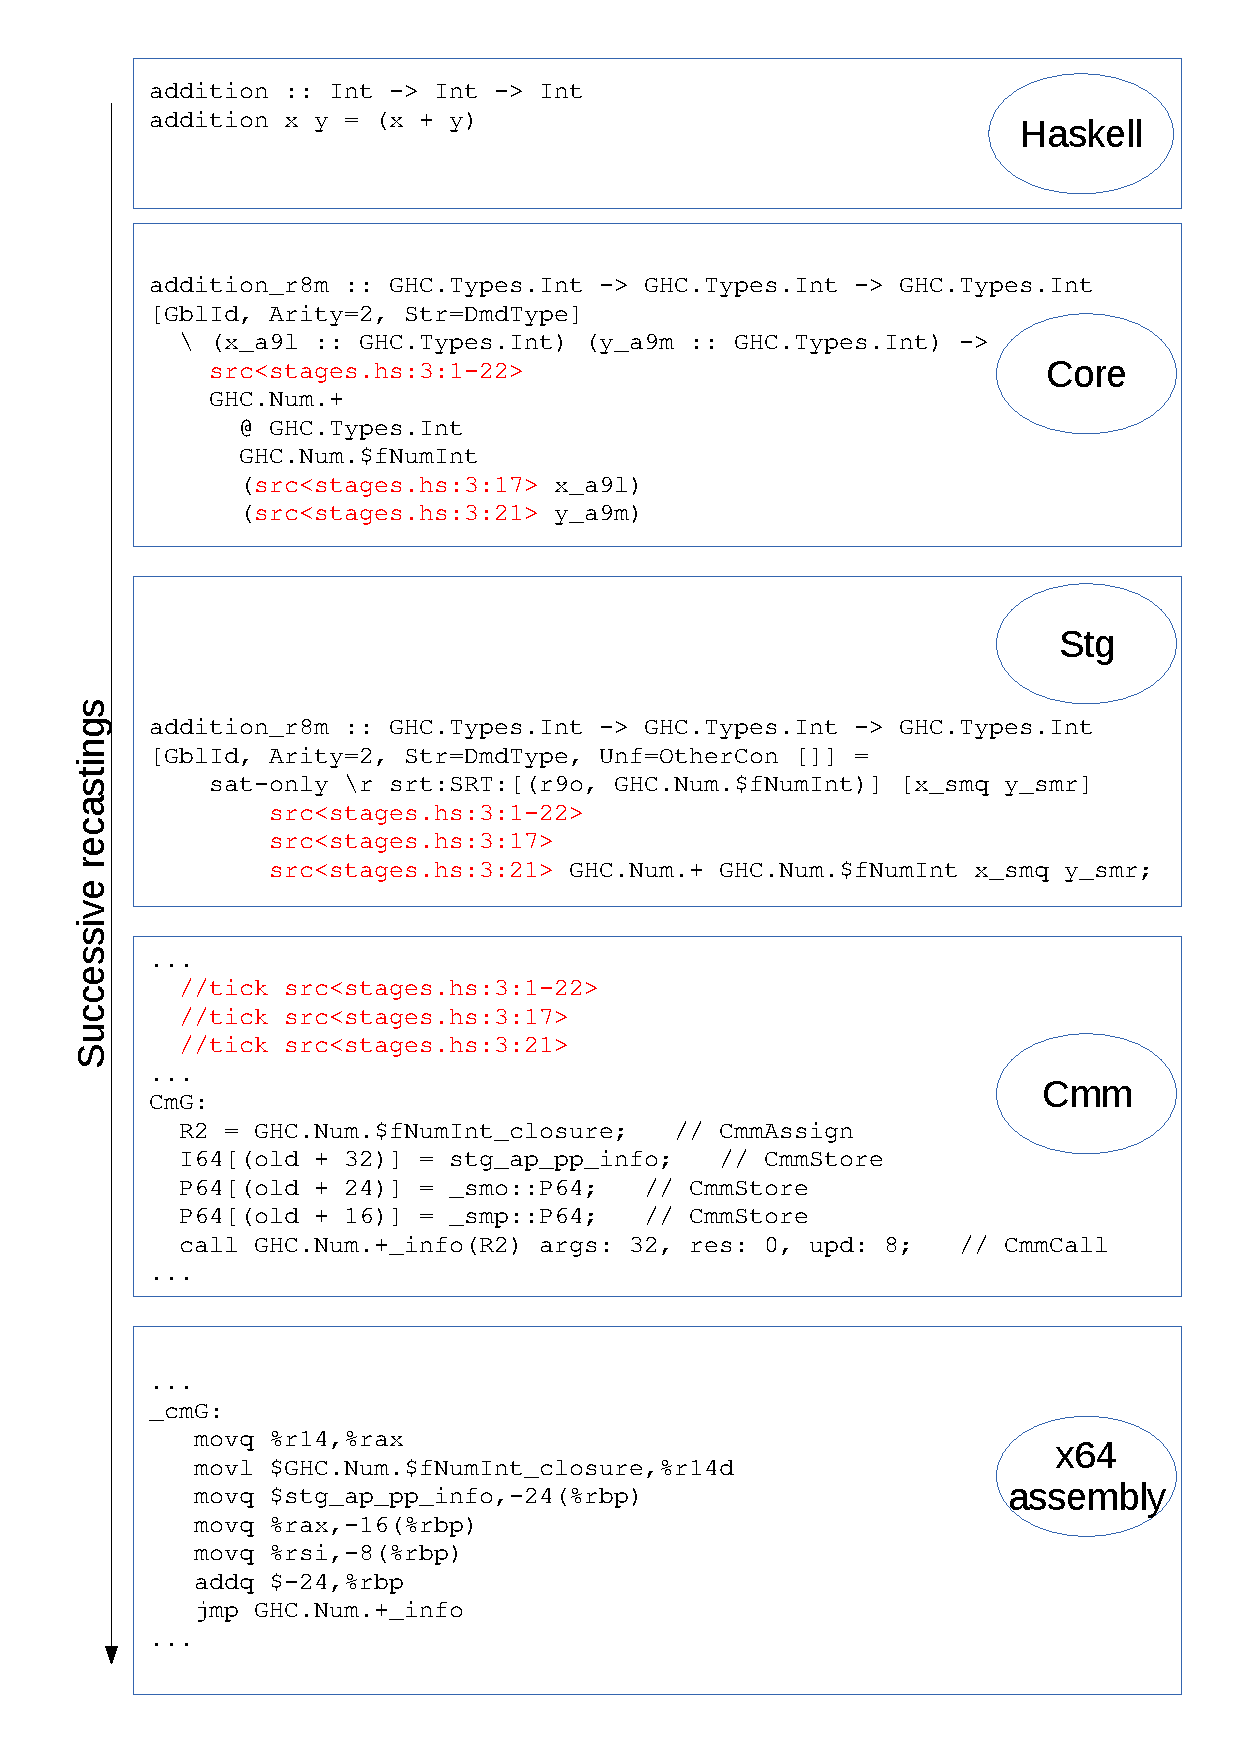
\includegraphics[width=5.4in]{fig/recastings_ticks}
  \caption{The same figure as~\ref{fig:recastings}, only that here each
  IR has debug data attached to it. The debug data tells us what Haskell
  source code the IR code is compiled from. For clarity the debug data
  annotations have a red font.}
  \label{fig:recastings_ticks}
\end{mdframed}
\end{figure}

One important observation is that
any implementation can only be a best effort implementation.
Consider figure~\ref{fig:same_functions} which contains two Haskell functions
with \emph{exactly} the same implementation. A clever compiler will
be able to realize that the two function bodies are identical,
it would then be safe for the compiler to remove one of the functions
and just change the call sites of the removed function to use the other function.
But this has a drawback because a stack trace
involving the removed function can not exist. Figure~\ref{fig:optimization} highlights this problem, Haskell can't
report which function caused the crash, since that
function is optimized away. In conclusion, an implementation of stack traces that have no
effect on performance can only be a best effort attempt.

\begin{figure}
\begin{mdframed}
  \begin{minted}{haskell}
kilometerToMeter = (*1000)
kilogramToGram = (*1000)
  \end{minted}
  \caption{Two functions with identical implementations. }
  \label{fig:same_functions}
\end{mdframed}
\end{figure}

\begin{figure}
\begin{mdframed}
        \begin{subfigure}[t]{0.5\textwidth}
            \begin{minted}{haskell}
reciprocal_1 :: Int -> Int
reciprocal_1 x = 1 `div` x

reciprocal_2 :: Int -> Int
reciprocal_2 = (1 `div`)

main = do
  print (reciprocal_1 5)
  print (reciprocal_2 0) -- crash!
            \end{minted}
            \caption{Original program.}
        \end{subfigure}
        ~ %add desired spacing between images, e. g. ~, \quad, \qquad etc.
          %(or a blank line to force the subfigure onto a new line)
        \begin{subfigure}[t]{0.5\textwidth}
          \begin{minted}{haskell}
reciprocal_1 :: Int -> Int
reciprocal_1 x = 1 `div` x

main = do
  print (reciprocal_1 5)
  print (reciprocal_1 0) -- crash!
          \end{minted}
          \caption{After optimizations.}
        \end{subfigure}
        \caption{An example showing why optimizations can give
        inaccurate stack traces.}\label{fig:optimization}
\end{mdframed}
\end{figure}

Finally, the information about the source-level functions that the compiler
has held tight throughout the IRs must get packaged into the binary. This
concern arises naturally in the final IR stage (Cmm in the case of GHC).  How does the compiler emit the
debug information? How is it stored in a way so it doesn't get in the way of the
actual code?  A debugging format answers these questions. One such debugging
format is DWARF.

\section{DWARF}

In 1988, DWARF was created hoping to solve a quite general problem. DWARF is
a language agnostic debugging format that is still producing updated revisions.
DWARF 5 is planned to be released in 2014 \cite{eager2012introduction}. The DWARF data that is
stored in the binary can be understood by a debugger like \texttt{gdb}. For example,
it could help \texttt{gdb} explain how some data should be displayed, for instance if a
particular byte is a 8-bit number or a character.

Looking at figure~\ref{fig:recastings_ticks} again, we see that neither
the first phase (the original Haskell source code) nor the last
phase (the output assembly) has any debug information attached to
it. This does make sense because programmers should not need to
annotate their source code to get stack traces, neither should the
performance of the program degrade by changing the output assembly.
But then where is the final debug data emitted? It must be included
with the binary of course. The binary is divided into \emph{sections}
\cite{oracle_object_file_format}, some of these sections are DWARF
sections. The command line tool \texttt{dwarfdump} can inspect the
DWARF data in object files. Figure~\ref{fig:dwarfdump} shows some of the
DWARF data that GHC included in the object file it created. The figure
shows only some of the relevant debug information, for example, the line
numbers are not stored anywhere in the contents of the figure.

\begin{figure}
\begin{mdframed}
  \begin{minted}{text}
< 1><0x0000008d>    DW_TAG_subprogram
                      DW_AT_name                  "addition"
                      DW_AT_MIPS_linkage_name     "r8m_info"
                      DW_AT_external              no
                      DW_AT_low_pc                0x00000020
                      DW_AT_high_pc               0x00000054
                      DW_AT_frame_base            DW_OP_call_frame_cfa
< 2><0x000000b3>      DW_TAG_lexical_block
                        DW_AT_name                  "cmG_entry"
                        DW_AT_low_pc                0x00000029
                        DW_AT_high_pc               0x0000004b
< 2><0x000000cf>      DW_TAG_lexical_block
                        DW_AT_name                  "cmF_entry"
                        DW_AT_low_pc                0x0000004b
                        DW_AT_high_pc               0x00000054
  \end{minted}
  \caption{The DWARF data generated from the debug annotations in figure~\ref{fig:recastings_ticks}.}
  \label{fig:dwarfdump}
\end{mdframed}
\end{figure}

As will be revealed in
section~\ref{sec:recent_work}, this thesis work was made possible thanks
to that DWARF got integrated in GHC.
